\chapter{Radiative corrections}
\setcounter{chapter}{6}
\section{Optical theorem}
We have seen in Advanced Quantum Theory that tree diagrams are in general \underline{real}. So there is no imaginary parts. Need to restore perturbatively in higher-order corrections. Then the optical theorem is valid again.

S-matrix is unitary: $S^\dagger S = \id$ with $S = \id + i T$. Thus
\begin{align*}
	-i (T - T^\dagger) = T^\dagger T
\end{align*}

We take matrix element for $k_1 k_2 \rightarrow p_1 p_2$ scattering. On RHS, insert a complete set of states,
\begin{align*}
	\braket{p_1 p_2 | T^\dagger T | k_1 k_2} = \sum_n \prod_{i=1}^n \int \frac{\dd^3 q_i}{(2\pi)^3 2 E_i} \braket{p_1 p_2 | T^\dagger | q_1 \dots q_n} \braket{q_1 \dots q_n | T | k_1 k_2}
\end{align*}

Reduce $T_{fi} = (2\pi)^4 \delta^{(4)}(p_f - p_i) M_{fi}$ and omitting overal $(2\pi)^4 \delta^{(4)}(p_f - p_i)$
\begin{align*}
	-i \left[ \M(k_1 k_2 \rightarrow p_1 p_2) - \M^* (p_1 p_2 \rightarrow k_1 k_2) \right]& \\
	= \underbrace{\sum \prod_{i=1}^n \int \frac{\dd^3 q_i}{(2\pi)^3 2 E_i}}_\text{invariant phase-space volume element} & \M^*(p_1 p_2 \rightarrow q_1 \dots q_n) \M(k_1 k_2 \rightarrow q_1 \dots q_n) (2\pi)^4 \delta^{(4)}(k_1 + k_2 - \sum_i q_i)
\end{align*}

So optical theorem, for forward scattering ($p_1 = k_1, p_2 =  k_2$) reads (see \ref{math:F})
\begin{align*}
	\Im \M(k_1 k_2 \rightarrow k_1 k_2) &= 2F \sigma_\text{tot} (k_1 k_2 \rightarrow \text{anything}) \\
	2\sqrt{s} |f_i^\text{CMS}| &= \lambda^{\frac{1}{2}} (s, m_1^2, m_2^2)
\end{align*}

\paragraph{Optical theorem for Feynman diagrams}
Consider a specific diagram contributing to the imaginary part, e.g.~in $\phi^4$-theory.
\begin{align}
	\feynmandiagram[small, baseline=(x.base), horizontal=x to y]{
		k1[particle=\(k_1\)] -- x --[quarter left] y -- p1[particle=\(p_1\)];
		k2[particle=\(k_2\)] -- x --[quarter right] y -- p2[particle=\(p_2\)];
	};
	p_s = k_1 + k_2 = p_1 + p_2, p_s^2 = s \notag\\
	i\M(s) = \frac{\lambda^2}{2} \int \frac{\dd^4 q}{(2\pi)^4} \frac{1}{ \left[ (p_s /2 - q)^2 - M^2 +i \epsilon \right] \left[ (p_s /2 + q)^2 - M^2 + i\epsilon \right] }\label{math:M}
\end{align}

From optical theorem: $\Im \M(s < 4M^2) = 0$, so $\M(s < 4M^2) \in \R$, (Since it is physical case, the cross section must vanish) when regarding $\M(s)$ as an analytic function of $s$ beyond what physical S-matrix element allow.

\paragraph{Schwarz reflection principle}
If (in some region) analytic function $\M(s)$ is \underline{real} at least for a finite, nonvanishing interval $\in \R$, then
\begin{align}
	\M(s^*) = \M^* (s)
\end{align}

Hence 
$$\M(s+i\epsilon)-\M(s-i\epsilon) \equiv \text{disc} \M(s) = \M(s + i\epsilon) - \M^*(s+i\epsilon) = 2i \Im \M(s+i\epsilon)$$
\begin{center}
\tikzset{zigzag/.style={decorate, decoration=zigzag}}
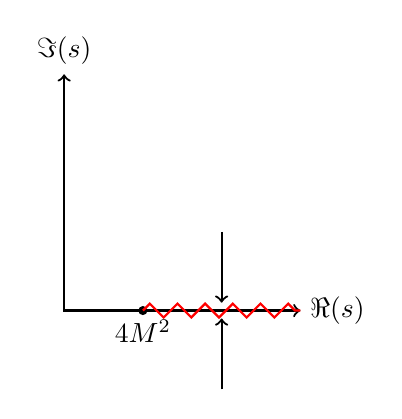
\begin{tikzpicture}[scale=1, transform shape]
	\draw [thick, <->] (0,3) -- (0,0) -- (3,0);
	\node [above] at (0,3) {$\Im(s)$};
	\node [right] at (3,0) {$\Re(s)$};
	\draw [fill] (1,0) circle [radius=0.05];
	\node [below] at (1,0) {$4M^2$};
	\draw [thick, zigzag, red] (1,0) -- (3,0);
	\draw [thick, ->] (2,1) -- (2,0.1);
	\draw [thick, ->] (2,-1) -- (2,-0.1);
\end{tikzpicture}
\end{center}

Onset of imaginary part for $s \leq 4M^2$ necessarily leads to a "branch cut", a nontrivial discontinuity in the comlex energy plane. The branch cut is equivalent to $\sqrt{4M^2 - s}$. Function has discontinuity, a cut, on real axis.

How can we calculate the discontinuity ($=$ imaginary part) of the above diagram?

Use centre-of-mass system $p_s = (\sqrt{s}, \pmb{0})$. Poles from propagators 
\begin{align*}
	& \frac{s}{4} \mp \sqrt{s}q^0 + q^2 - M^2 + i\epsilon = 0  \\
	\Leftrightarrow &(q^0)^2 \pm \sqrt{s} q^0 + \frac{s}{4} - |\pmb{q}|^2 -M^2 + i\epsilon = 0
\end{align*}

\begin{align*}
	& \text{first propagator} && q^0 = + \frac{\sqrt{s}}{2} \pm (\sqrt{M^2 + |\pmb{q}|^2} - i\epsilon) = +\frac{\sqrt{s}}{2} \pm (E_q - i\epsilon) \\
	& \text{second propagator} && q^0 = -\frac{\sqrt{s}}{2} \pm (E_q - i\epsilon)
\end{align*}

\begin{center}
\tikzset{zigzag/.style={decorate, decoration=zigzag}}
\begin{tikzpicture}[scale=1, transform shape]
	\draw [thick, <->] (0,2) -- (0,0) -- (5,0);
	\draw [thick] (0,-2) -- (0,0) -- (-5,0);
	\node [above] at (0,2) {$\Im(q^0)$};
	\node [right] at (5,0) {$\Re(q^0)$};
	\node [above] at (-2,0.5) {$+\frac{\sqrt{s}}{2} - E_q + i\epsilon$};
	\draw [fill] (-2,0.5) circle [radius=0.05];
	\node [above] at (-5,0.5) {$-\frac{\sqrt{s}}{2} - E_q + i\epsilon$};
	\draw [fill] (-5,0.5) circle [radius=0.05];
	\node [below] at (2,-0.5) {$-\frac{\sqrt{s}}{2} + E_q + i\epsilon$};
	\draw [fill] (2,-0.5) circle [radius=0.05];
	\node [below] at (5,-0.5) {$+\frac{\sqrt{s}}{2} + E_q + i\epsilon$};
	\draw [fill] (5,-0.5) circle [radius=0.05];
\end{tikzpicture}
\end{center}

If we close the contour of the $q_0$ integration in the \underline{lower} half plane, we only pick up the 2 residues at $\mp \frac{\sqrt{s}}{2}+E_q -i\epsilon$. As $E_q$ is positive, only $-\frac{\sqrt{s}}{2} + E_q -i \epsilon$ from second propagator contirbutes to discontinuity. So pinching up the residue equivalent to replacement under $q^0$ integration
\begin{align*}
	\frac{1}{(p_s /2 + q)^2 - M^2 +i\epsilon} \longmapsto  \underbrace{-2\pi i}_{\text{orientation of contour}} \delta((p_s / 2 + q)^2 - M^2)
\end{align*}

Determine the residue of the rest at the pole at $-\frac{\sqrt{s}}{2} + E_q  - i\epsilon$
\begin{align}
	M(s) \longmapsto &-\frac{\lambda^2}{2} \int \frac{\dd^3 q}{(2\pi)^3} \frac{1}{2E_q \sqrt{s}(\sqrt{s}-2E_q)} \notag \\
	\shortintertext{With no angular dependence and using substitution (note the limits of integral also change)$\dd^3 q \rightarrow 4 \pi |\pmb{q}|^2 \dd |\pmb{q}| = 4 \pi |\pmb{q}|E_q \dd E_q$}
	& = -\frac{\lambda^2}{8\pi^2} \int^\infty_M \frac{\dd E_q \sqrt{E_q^2 - M^2}}{\sqrt{s}(\sqrt{s} - 2E_q)}  \label{math:res}
\end{align}

It has pole at $E_q = \frac{\sqrt{s}}{2}$. The second pole in \ref{math:M} at $\frac{\sqrt{s}}{2} + E_q - i\epsilon$ would produce a pole in \ref{math:res} for $E_q = -\frac{\sqrt{s}}{2}$, outside the integration range $M \leq E_q < \infty$.

\begin{itemize}
	\item for $\sqrt{s} < 2M$, \ref{math:res} is manifestly real.
	\item for $\sqrt{s} > 2M$, the pole at $E_q = \frac{\sqrt{s}}{2}$ in \ref{math:res} contributes \underline{differently} depending on $\sqrt{s}\pm i\epsilon$; difference yields discontinuity.
\end{itemize}
Use
\begin{align*}
	\frac{1}{\sqrt{s}-2E_q\pm i\epsilon} = \underbrace{\frac{P}{\sqrt{s} - 2 E_q}}_{\text{real}} \underbrace{\mp i\pi \delta(\sqrt{s} - 2 E_q)}_{\text{yields discontinuity}}
\end{align*}

So for calculation of the discontinuity, have replacement 
\begin{align*}
	\frac{1}{(p_s/2 - q)^2 - M^2 + i\epsilon} \longmapsto -2\pi i \delta((p_s/2 -q)^2 - M^2)
\end{align*}
for other propagator too!

\paragraph{Cuthosky rules (1960)} replace cut propagator according to 
\begin{align}
	\frac{1}{p^2 - M^2 + i\epsilon} \longmapsto -2\pi  i \delta(p^2 - M^2)
\end{align}
to calculate discontinuity across the cut!

Calculateion completed:
\begin{align*}
	\text{disc} \left(	
		\feynmandiagram[small, baseline=(x.base), horizontal=x to y]{
			k1 -- x --[quarter left] y -- p1;
			k2 -- x --[quarter right] y -- p2;
		};
	\right )
	 &= i\frac{\lambda^2}{2} \int \frac{\dd^4 q}{(2\pi)^4} 2\pi \delta(q^2 - M^2) 2\pi \delta((p_s - q)^2 - M^2) \\
	 \shortintertext{using $\dd^4 q = \dd q^0 \dd q |q|^2 \dd \Omega_q$ and $(p_s - q)^2 - M^2 = s - 2\sqrt{s}q^0$}
	 &= \frac{\lambda^2}{2} \frac{i}{4\pi^2} \int \frac{|q|^2 \dd |q| \dd \Omega_q}{2q^0} \delta(s - 2\sqrt{s}q^0) \\
	 &= \frac{\lambda^2}{2} \frac{i}{8\pi^2} \int \sqrt{(q^0)^0 - M^2} \dd q^0 \dd \Omega_q \delta(s - 2\sqrt{s}q^0) \\
	 &= \frac{\lambda^2}{2} \frac{i}{8\pi^2} \frac{\sqrt{s/4 - M^2}}{2\sqrt{s}} \int \dd \Omega_q \\
	 &= \frac{\lambda^2}{2} \frac{i}{8\pi} \sqrt{1 - \frac{4M^2}{s}} \\
	\text{Im}\M &= \frac{\lambda^2}{4} \frac{1}{8\pi} \sqrt{1 - \frac{4M^2}{s}}
\end{align*}
Note $\sigma = \frac{\lambda^2}{32\pi}$ and $2F = s \sqrt{1-\frac{4M^2}{s}}$. Thus optical theorem is still valid.

We can do more. Construct the complete $\M(s)$ from $\Im\M(s)$ through a \underline{dispersion relation}!

\begin{center}
\tikzset{zigzag/.style={decorate, decoration=zigzag}}
\usetikzlibrary{decorations.markings}
\tikzset{decoration={
    markings,
    mark=at position 0.5 with {\arrow{>}}}}
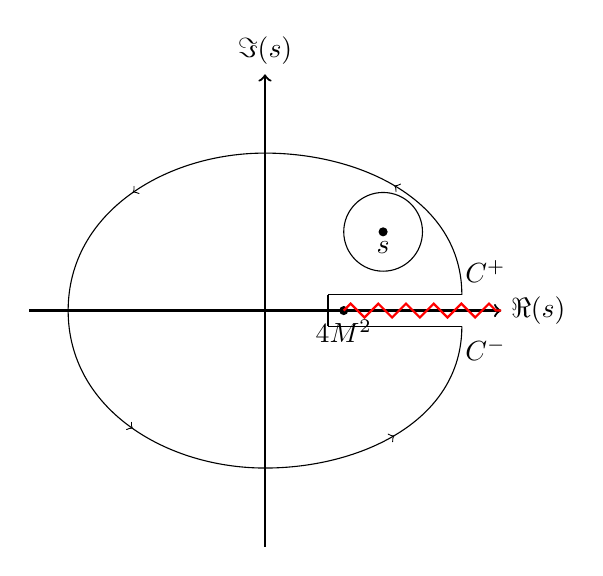
\begin{tikzpicture}[scale=1, transform shape]
	\draw [thick, <->] (0,3) -- (0,0) -- (3,0);
	\draw [thick, -] (0,-3) -- (0,0) -- (-3,0);
	\node [above] at (0,3) {$\Im(s)$};
	\node [right] at (3,0) {$\Re(s)$};
	\draw [fill] (1,0) circle [radius=0.05];
	\node [below] at (1,0) {$4M^2$};
	\draw [thick, zigzag, red] (1,0) -- (3,0);

	\draw [fill] (1.5,1) circle [radius=0.05];
	\draw (1.5,1) circle [radius=0.5];
	\node [below] at (1.5,1) {$s$};
	\draw[postaction={decorate}] (2.5,0.2) to [out=90, in=0] (0,2);
	\draw[postaction={decorate}] (0,2) to [out=-180, in=90] (-2.5,0);
	\draw[postaction={decorate}] (0,-2) to [out=0, in=-90] (2.5,-0.2);
	\draw[postaction={decorate}] (-2.5,0) to [out=-90, in=180] (0,-2) ;

	\draw (0.8,0.2) -- (2.5,0.2);
	\draw (0.8,-0.2) -- (2.5,-0.2);
	\draw (0.8, 0.2) -- (0.8, -0.2);

	\node at (2.8,0.5) {$C^+$};
	\node at (2.8,-0.5) {$C^-$};
\end{tikzpicture}
\end{center}

Use Cauchy's theorem:
\begin{align}
	\M(s) &= \frac{1}{2\pi i} \oint \frac{\M(z)\dd z}{z-s} \\
	\shortintertext{dropping the large circle}
		  &\longmapsto  \frac{1}{2\pi i }\int_{C_+ + C_-} \frac{\M(z)\dd z}{z-s}\notag\\
	&= \frac{1}{2 \pi i} \left[ \int^\infty_{4M^2}\frac{M(z+i\epsilon)\dd z}{z-s} - \int^\infty_{4M^2}\frac{M(z-i\epsilon)\dd z}{z-s} \right] \notag\\
	&= \frac{1}{2\pi i }\int^\infty_{4M^2} \frac{\text{disc}\M(z)\dd z}{z -s } \notag\\
	&= \frac{1}{\pi} \int^\infty_{4M^2} \frac{\Im\M(z) \dd z}{z-s} 
\end{align}

Repeat the exercise for $\frac{\M(s)-\M(0)}{s}$ (no pole introduced!).
\begin{align*}
	\Im \left( \frac{\M(s)-\M(0)}{s} \right) &= \frac{\Im\M(s)}{s} \\
	\M(s) - \M(0) &= \frac{s}{\pi} \int^\infty_{4M^2} \frac{\Im\M(z)\dd z}{z(z-s)} \\
				  &= \frac{\lambda^2}{2} \frac{s}{(4\pi)^2} \int^\infty_{4M^2} \frac{\dd z}{z(z-s)} \sqrt{1-\frac{4M^2}{z}} \\
	\shortintertext{using $\sigma = \sqrt{1-\frac{4M^2}{s}}$ and $\zeta = \sqrt{1 - \frac{4M^2}{z}}$}
				&= \frac{\lambda^2}{2}\frac{1}{8\pi^2} \int^1_0 \frac{\zeta^2}{\zeta^2 - \sigma^2} \dd \zeta \\
				&= \frac{\lambda^2}{2}
	\begin{cases}
		\frac{1}{8\pi^2} \left( 1 -\frac{\sigma}{2}\log{\frac{\sigma+1}{\sigma-1}} \right) & s < 0 \Leftrightarrow \sigma > 1 \\
		\frac{1}{8\pi^2} \left( 1- \sqrt{-\sigma^2} \arctan{\frac{1}{\sqrt{-\sigma^2}}} \right) & 0 < s < 4M^2, \sigma^2 < 0 \\
		\frac{1}{8\pi^2} \left( 1 - \frac{\sigma}{2}\log{\frac{1+\sigma}{1-\sigma}} + \frac{\textcolor{red}{i}\sigma}{16\pi} \right) & s > M^2, 0 < \sigma < 1
	\end{cases}
\end{align*}

Note: we are going to calculate this diagram again, noticing that $\int \frac{\dd^4 q}{(q^2 \dots)(q^2 \dots)}$ is logarithmically divergent!. The above representation demonstrates that this divergence resides in $M(0)$!

\section{Field-strength renomrlization}
What is structure of the propagator $\braket{\Omega | T\phi(x)\phi(y) | \Omega}$ at higher orders? At lower order
\begin{align*}
	\feynmandiagram[small, horizontal=a to b]{a --[fermion, edge label=\(p\)]b;};
	= \frac{i}{p^2 - M^2 + i\epsilon}
\end{align*}
Beyond this the propagator is not a simple pole. In $\phi^3$-theory 
\feynmandiagram[layered layout, small, horizontal=a to b, baseline=(a.base)]{
	a -- x;
	x --[half left] y;
	x --[half right] y;
	y -- b;
};
branch cuts are at $p^2 \leq 4M^2$.
In $\phi^4$-theory
\feynmandiagram[layered layout, small, horizontal=a to b, baseline=(a.base)]{
	a -- x;
	x --[half left] y;
	x --[half right] y;
	x -- y;
	y -- b;
};	
branch cuts are at $p^2 \leq 9M^2$. To induce cuts in the analytic structure.

Insert complete set of intermediate states ($x^0 > y^0$)
\begin{align*}
	\braket{\Omega | T\phi(x)\phi(y) | \Omega} = \sum_\lambda \int \frac{\dd^3 p}{(2\pi)^3 2E_p(\lambda)} \braket{\Omega | \phi(x) | \lambda_{\pmb{p}}} \braket{\lambda_{\pmb{p}} | \phi(y) | \Omega}
\end{align*}
with
\begin{itemize}[label={}]
	\item $\lambda$ multiparticle state
	\item $\lambda_0$ "rest frame", i.e.~$\hat{\pmb{P}}\ket{\lambda_0} = 0$
	\item $\lambda_{\pmb{p}}$ boosted to momentum $\pmb{p}$
\end{itemize}

Call energy of $\lambda_0 = m_\lambda$. From single particle to multi particle $E_{\pmb{p}}(\lambda) = \sqrt{m^2_\lambda + |\pmb{p}|^2}$.

\begin{align*}
	\braket{\Omega | \phi(x) | \lambda_{\pmb{p}}} &= \braket{\Omega| e^{i\hat{P}x} \phi(0) e^{-i\hat{P}x}|\lambda_{\pmb{p}}}	\\
									   &= \left. \braket{\Omega| \phi(0) | \lambda_{\pmb{p}}} e^{-ipx} \right\rvert_{p^0 = E_{\pmb{p}}} \\
									   \shortintertext{$\Omega$ and $\phi(0)$ are invariant under momentum boost}
									   &= \left. \braket{\Omega| \phi(0) | \lambda_{0}} e^{-ipx} \right\rvert_{p^0 = E_{\pmb{p}}} \\
\end{align*}

\begin{align}
	\braket{\Omega | T\phi(x)\phi(y) | \Omega} &= \sum_\lambda \int \frac{\dd^3 p}{(2\pi)^3 2E_p(\lambda)} e^{-ip(x-y)} |\braket{\Omega| \phi(0) | \lambda_0 }|^2 \\
											   &= \sum_\lambda \underbrace{\int \frac{\dd^4 p}{(2\pi)^4} \frac{i}{p^2 - m^2_\lambda + i\epsilon} e^{-ip(x-y)}}_{D_F(x-y;m^2_\lambda) \text{ when combined with } y^0 > x^0} |\braket{\Omega| \phi(0) | \lambda_0 }|^2 \\ 
\end{align}

Formally write this as 
\begin{align}
	\braket{\Omega | T\phi(x)\phi(y) | \Omega} = \int^\infty_0 \frac{\dd s}{2\pi} \rho(s) D_F(x-y;s)
\end{align}
with $\rho(s)$ the spectral density function.
\begin{align}
	\rho(s) \defeq \sum_\lambda (2\pi) \delta(s - m_\lambda^2) \left| \braket{\Omega | \phi(0) | \lambda_0} \right|^2
\end{align}

A typical spectral function looks like
\begin{figure}[htpb]
\begin{center}
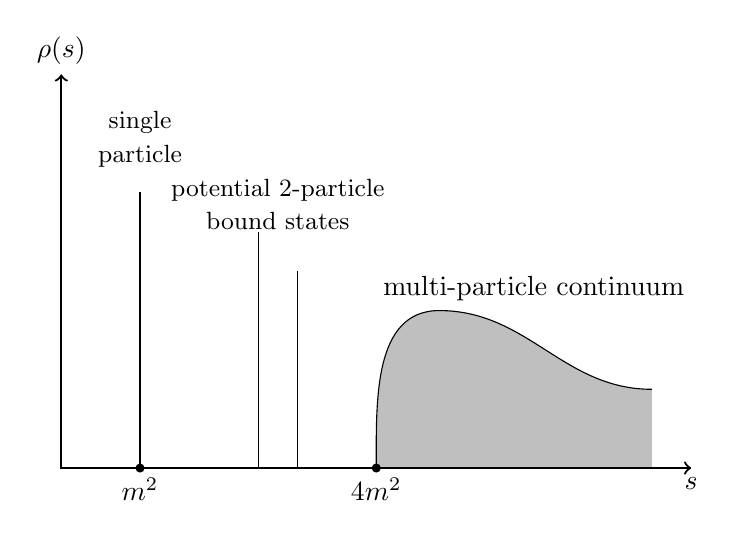
\begin{tikzpicture}[scale=1, transform shape]
	\draw [fill] (1,0) circle [radius=0.05];
	\node [below] at (1,0) {$m^2$};
	\draw (1,3.5) -- (1,0);
	\node [above, align=center] at (1,3.7) {\small single\\ \small particle};

	\draw (3,2.5) -- (3,0);
	\draw (2.5,3) -- (2.5,0);
	\node [above, align=center] at (2.75, 2.9) {\small potential 2-particle \\ \small bound states};

	\draw [draw opacity=0, fill=lightgray] (4,0) to [out=90, in=180] (4.8,2) to [out=0, in=180] (7.5,1) -- (7.5,0) ;
	\draw (4,0) to [out=90, in=180] (4.8,2) to [out=0, in=180] (7.5,1);
	\draw [fill] (4,0) circle [radius=0.05];
	\node [below] at (4,0) {$4m^2$};
	\node [above] at (6, 2) {multi-particle continuum};

	\draw [thick, <->] (0,5) -- (0,0) -- (8,0);	
	\node [above] at (0,5) {$\rho(s)$};
	\node [below] at (8,0) {$s$};
\end{tikzpicture}
\end{center}
\caption{typical spectral function}
\label{fig:specFunc}
\end{figure}

Single particle contribution
\begin{align}
	\rho(s) = 2\pi \delta(s-m^2)Z + (\text{contributions} \geq 4m^2)
\end{align}
with $Z = \left| \braket{\Omega | \phi(0) | \lambda_{0}}\right|^2$ the field-strength renomrlization factor. 

Fourier transforming two-point function
\begin{align*}
	&\int \dd^4 x e^{ipx} \braket{\Omega | T\phi(x)\phi(0) | \Omega} \\
	=& \int^\infty_0 \frac{\dd s}{2\pi} \rho(s) \frac{i}{p^2 - s + i\epsilon} \\
	=& \frac{iZ}{p^2 - m^2 _ i\epsilon} + \int^\infty_{\sim 4m^2} \frac{\dd s}{2\pi} \rho(s) \frac{i}{p^2 - s + i\epsilon}
\end{align*}

Comparing to free theory: $\braket{0| \phi(0) | \pmb{p}}=1$ hence $Z=1$.

\section{LSZ reduction formula}

\section{The propagator(again)}
See also Peskin \& S. Chapter 10.2.

How do we calculate the propagtor and the wave-function renormalization factor $Z$ in perturbation theory, using Feynman diagrams? Call mass \underline{parameter} in $\lag = \frac{1}{2}(\partial_\mu \phi_0)^2 - \frac{m^2_0}{2}\phi_0^2 - \frac{\lambda_0}{4!}\phi_0^4$ $m_0$ \textit{bare mass}.

In $\phi^4$-theory "1-particle-irreducible" (1PI) contribution is
\begin{align*}
	-i\Sigma(p^2) = &
	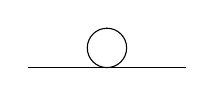
\begin{tikzpicture}[scale=1, transform shape]
		\draw (0,0) -- (2,0);
		\draw (1,0.25) circle[radius=0.25];
	\end{tikzpicture} 
	+
	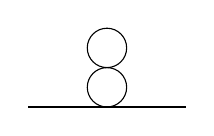
\begin{tikzpicture}[scale=1, transform shape]
		\draw (0,0) -- (2,0);
		\draw (1,0.25) circle[radius=0.25];
		\draw (1,0.75) circle[radius=0.25];
	\end{tikzpicture}
	+ 
	\begin{tikzpicture}[scale=1, transform shape,baseline=(a.base)]
		\draw (a) (0,0) -- (2,0);
		\draw (1,0) circle[radius=0.5];
	\end{tikzpicture}
	+ \dots \\
	\shortintertext{Then the \underline{complete} propagator using $D^0_F(p^2) = \frac{i}{p^2 - m^2_0 +i\epsilon}$ is} 
	D_F(p^2) =& 
	\begin{tikzpicture}[scale=1, transform shape]
		\draw (0,0) -- (2,0);
	\end{tikzpicture} 
	+
	\begin{tikzpicture}[scale=1, transform shape,baseline=(a.base)]
		\draw (a) (0,0) -- (0.6,0);
		\draw (a) (1.4,0) -- (2,0);
		\draw (1,0) circle[radius=0.4];
		\node at (1,0) {$-i\Sigma$};
	\end{tikzpicture}
	+
	\begin{tikzpicture}[scale=1, transform shape,baseline=(a.base)]
		\draw (a) (-0.2,0) -- (0.2,0);
		\draw (0.6,0) circle[radius=0.4];
		\node at (0.6,0) {$-i\Sigma$};
		\draw (1,0) -- (1.2,0);
		\draw (1.6,0) circle[radius=0.4];
		\node at (1.6,0) {$-i\Sigma$};
		\draw (2,0) -- (2.4,0);
	\end{tikzpicture} \\
	=& D^0_F(p^2) + D_F^0 (p^2) \left( -i\Sigma(p^2) \right)D^0_F(p^2)  +  D_F^0 (p^2) \left( -i\Sigma(p^2) \right) D_F^0 (p^2) \left( -i\Sigma(p^2) \right) D^0_F(p^2) \\
	\shortintertext{It is cleary a geometric series}
	=& \frac{D^0_F(p^2)}{1+i\Sigma(p^2)D_F^0(p^2)} = \frac{i}{p^2 - m_0^2 -\Sigma(p^2)}
\end{align*}
The pole of propagator does not occur at $m_0^2$ anynore. It will be shifted by $\Sigma \sim \mathcal{O}(\lambda)$!

Choose $m^2$ by the condition 
\begin{align}
	m_0^2 + \Sigma(m^2) = m^2
\end{align}
Expand
\begin{align}\label{math:Sigma}
	\Sigma(p^2) = \Sigma(m^2) + (p^2 - m^2) \Sigma'(m^2) + (p^2 - m^2)\tilde{\Sigma}(p^2)
\end{align}
where $\tilde{\Sigma}$ represents a correction (to first order Taylor expansion) and it satisfies $\tilde{\Sigma}(m^2) = 0$.

Then the propagator
\begin{align}
	D_F(p^2) =& \frac{i}{p^2 - m^2_0 - \Sigma(p^2)} = \frac{i}{(p^2 - m^2)(1+\frac{\Sigma(m^2)-\Sigma(p^2)}{p^2 - m^2})} \notag \\
	\shortintertext{using \ref{math:Sigma}}
	=& \frac{i}{(p^2 - m^2)(1-\Sigma'(m^2)-\tilde{\Sigma}(p^2))} \notag\\
	=& \frac{iZ}{p^2 - m^2} \cdot \frac{1}{1-Z\tilde{\Sigma}(p^2)} \notag \\
	=& \frac{iZ}{p^2 - m^2} + \text{regular}
\end{align}
with $Z = \left( 1 - \frac{\partial}{\partial p^2} \left.\Sigma(p^2)\right\rvert_{p^2 = m^2} \right)^{-1}$

Starting point Lagrangian is $\lag = \frac{1}{2}(\partial_\mu \phi_0)^2 - \frac{m^2_0}{2}\phi_0^2 - \frac{\lambda_0}{4!}\phi_0^4$. To remove $Z$ from numerator frome the propagator and instead put $\sqrt{Z}$ onto the couplings at each end. Since each internal vertex has 4 lines (remember the vertex carries the coupling constant)
\begin{align}
	\lambda_0 \longmapsto \lambda_1 = Z^2 \lambda_0
\end{align}

In $\Sigma$ and $\tilde{\Sigma}$, there are 2 external lines without $\sqrt{Z}$, so
\begin{align}
	\Sigma(p^2, \lambda_0, \text{old } D_F) = \frac{1}{Z} \Sigma_1(p^2, \lambda_1, \text{new } D'_F)
\end{align}
(same expression for $\tilde{\Sigma}$).

Thus we get the new propagator
\begin{align}
	D'_F(p^2) = \frac{i}{p^2 - m^2} \cdot \frac{1}{1-\tilde{\Sigma}_1(p^2)}
\end{align}
where $\tilde{\Sigma}_1(m^2) = 0$.

Define the renomalized field
\begin{align}
	Z^{-\frac{1}{2}} \phi_0 = \phi
\end{align}
Then $D'_F$ is the Fourier transform of $\braket{0 | T\phi(x)\phi(y) | 0}$

Rewrite the Lagrangian as
\begin{align}
	\lag = \frac{1}{2} \left( (\partial_\mu \phi)^2 - m^2 \phi^2 \right) \boxed{-\frac{\lambda_1}{4!}\phi^4 \underbrace{- \frac{1}{2}\delta m^2 \phi^2 + \frac{1}{2}(Z-1) \left( (\partial_\mu \phi)^2 - m^2 \phi^2 \right)}_{\text{counter-terms}} }
\end{align}
where $\delta m^2 = -Z(m^2 + m_0^2) = -Z\Sigma(m^2) = -\Sigma_1 (m^2)$. Everythin inside the $\boxed{\text{box}}$ can be considered as "interaction". May look weird given the kinetic/mass-like terms, but no contradiction. Consider just $\lag = \frac{1}{2}(\partial \phi)^2 - \frac{m^2}{2}\phi^2$. The mass-term $\equiv$ "interaction".

A massless propagator $\feynmandiagram[small, horizontal=a to b, baseline=(a.base)]{a--b}; = \frac{i}{p^2}$ and interaction $\feynmandiagram[small, horizontal=a to b, baseline=(a.base)]{a --[insertion=0.5] b;};=-im^2$. The resummed propagator is then
\begin{align*}
	\feynmandiagram[layered layout, horizontal=a to x, small, baseline=(x.base)]{
		a -- x[blob] -- b;
	};
	=&
	\feynmandiagram[small, horizontal=a to b, baseline=(a.base)]{a --b;};
	+
	\feynmandiagram[small, horizontal=a to b, baseline=(a.base)]{a --[insertion=0.5] b;};
	+
	\feynmandiagram[small, horizontal=a to b, baseline=(a.base)]{a --[insertion=0.33, insertion=0.66] b;};
	+ \dots \\
	=& \frac{i}{p^2} \left( 1 + \frac{i}{p^2}\cdot(-im^2)+\dots \right) \\
	=& \frac{i}{p^2} \left( 1 - (-im^2)\frac{i}{p^2} \right)^{-1} = \frac{i}{p^2 - m^2} 
\end{align*}

Actually this is not all. We will also have to further renomalize $\lambda_1$
\begin{align*}
	\begin{tikzpicture}[scale=1, transform shape, baseline=(x.base)]
		\begin{feynman}
			\vertex (x1);
			\vertex (x2) at (2,0);
			\vertex (x3) at (0,-2);
			\vertex (x4) at (2,-2);
			\vertex (x) at (1,-1);
			\diagram*{
				(x1)-- (x) --(x2),
				(x3)-- (x) --(x4),
			};
		\end{feynman}
	\end{tikzpicture}
	+
		\begin{tikzpicture}[scale=1, transform shape, baseline=(x.base)]
		\begin{feynman}
			\vertex (x1);
			\vertex (x2) at (2,0);
			\vertex (x3) at (0,-2);
			\vertex (x4) at (2,-2);
			\vertex (xx) at (1,-0.6);
			\vertex (y) at (1,-1.4);
			\diagram*{
				(x1)-- (xx) --(x2),
				(x3)-- (y) --(x4),
				(xx) --[quarter left] (y) --[quarter left] (xx),
			};
		\end{feynman}
	\end{tikzpicture}
	+
	\begin{tikzpicture}[scale=1, transform shape, baseline=(x.base)]
		\begin{feynman}
			\vertex (x1);
			\vertex (x2) at (2,0);
			\vertex (x3) at (0,-2);
			\vertex (x4) at (2,-2);
			\vertex (x) at (0.6,-1);
			\vertex (y) at (1.4,-1);
			\diagram*{
				(x1)-- (x) --(x3),
				(x2)-- (y) --(x4),
				(x) --[quarter left] (y) --[quarter left] (x),
			};
		\end{feynman}
	\end{tikzpicture}
	+
	\begin{tikzpicture}[scale=1, transform shape, baseline=(x.base)]
		\draw (0,0) to  (0.6,-0.5) to[out=-45, in=45] (0.6, -1.5) to (0,-2);
		\draw (0.6, -0.5) to [out=180, in=-180] (0.6,-1.5);
	\end{tikzpicture}
\end{align*}

%%%%%%%%%%%%%%%%%%% TODO: complete the rest

%%%%%%%%%%%%%%%%%%%%%%%%%%%%%%%%%%%%%%%%%%%
\begin{align*}
	\begin{tikzpicture}[scale=1, transform shape, baseline=(x.base)]
		\begin{feynman}
			\vertex (x1);
			\vertex (x2) at (2,0);
			\vertex (x3) at (0,-2);
			\vertex (x4) at (2,-2);
			\vertex (x) at (0.6,-1);
			\vertex (y) at (1.4,-1);
			\diagram*{
				(x1)-- (x) --(x3),
				(x2)-- (y) --(x4),
				(x) --[quarter left] (y) --[quarter left] (x),
			};
		\end{feynman}
	\end{tikzpicture}
	= \frac{\mu^{2(4-d)\lambda^2}\lambda^2}{2} \int^1_0 \dd x \int \frac{\dd^d k}{(2\pi)^d} \frac{1}{[k^2 - \Delta(x)]^2} \\
	= \frac{\lambda^2}{2} \mu^{2(4-d)} \int_0^1 \dd x \frac{1}{(4\pi)^{d/2}} \frac{\Gamma(2-d/2)}{\Gamma(2)} \frac{1}{\Delta(x)^(2-d/2)} \\
	= \frac{\lambda^2}{2} \frac{\mu^{4-d}}{(4\pi)^2} \left\{ -2 \left[ \frac{1}{d-4} + \frac{1}{2}(\gamma_E - \log{4\pi} + \log(\frac{M}{\mu})) \right] - \int^1_0 \dd x \log{\frac{\Delta(x)}{M^2}} \right\} \quad \Delta(x)= M^2 - x(1-x)p^2 \\ 
	\int_0^1 \dd x \log{\frac{M^2-x(1-x)p^2}{M^2}} = \int_0^1 \dd x \log{ \left[ (\frac{\sigma+1}{2} - x)(x+\frac{\sigma-1}{2}) \right] } - \log{\frac{\sigma^2 - 1}{4}} , \quad \sigma = \sqrt{1-\frac{4M^2}{p^2}} \\
	= \sigma \log{\frac{\sigma+1}{\sigma-1}} - 2
\end{align*}
Valid for $p^2 < 0$, rest by analytic contination

Compare $M(s) - M(0)$ calculated based on Cutkosky and dispersion integral. Easier 
\begin{align*}
	M(0) = \frac{1}{i} \int \frac{\dd^d k}{(2\pi)^d} \frac{1}{(k^2 - M^2)^2} = \frac{\partial}{\partial M^2} \frac{1}{i} \int \frac{\dd^d k}{(2\pi)^d} \frac{1}{k^2 - M^2} \\
	= \frac{\partial}{\partial M^2} \left\{ -\frac{M^2}{8\pi^2} \left[ \frac{1}{d-4} + \frac{1}{2}(\gamma_E - 1 -\log{4\pi}) + \frac{1}{2} \log{\frac{M^2}{\mu^2}} \right] \right\} \\
	\shortintertext{$1$ cancalled by the derivative of $\log$}
	= - \frac{1}{8\pi^2} \left[ \frac{1}{d-4} + \frac{1}{2} (\gamma_E - \log(4\pi) + \frac{1}{2} \log{\frac{M^2}{\mu^2}}) \right]
\end{align*}

Lets summarise the renormalization of $\phi^4$ at one loop
\begin{itemize}
	\item   %TODO diagram
		is \underline{indeoendt} of $p^2$! Hence $\Sigma(p^2)$ at $\mathcal{O}(\lambda)$ only renormalises the \underline{mass}, there is no wavefunction renormalisation $Z (\sim \frac{\partial \Sigma}{\partial p^3} |_{p^2 = M^2})$. Thus $Z=1 + \mathcal{O}(\lambda^2)$
	This does change at $\mathcal{O}{\lambda^2}$: % TODO: diagram 
	$\rightarrow Z\neq 1$
\item Mass renomalisation
	% TODO: diagram
	Then 
	\begin{align*}
	M^2 = M^2 + \frac{\lambda M^2}{16\pi^2} \left[ \frac{1}{d-4} + \frac{1}{2} (\gamma_E - 1 -\log{4\pi} + \log{\frac{M}{\mu}}) \right]- M^2 + M^2 \\
	= M^2_0 + \frac{\lambda M^2}{16\pi^2} \left[ \frac{1}{d-4}  + \frac{1}{2}(\gamma_E - 1 - \log{4\pi} + \log{\frac{M}{\mu}}) + \mathcal{O}(\lambda, (d-4)) \right] \\
	M^2_\text{physical} \neq f(\mu), \quad \lambda \mu^{4-d} M^2 = \lambda_0 M_0^2 + \mathcal{O}(\lambda^2) \text{ and $\lambda_0$ and $M_0$ are independent of $\mu$}
	\end{align*}
	\item Coupling constant renormlaisation. Lets choose renormlisation point for $\lambda$ at $s=t=u=0$ for simplicity:
		%TODO: diagram
		with $Z=1$
		\begin{align*}
			\lambda_0 =  \lambda \mu^{4-d}Z_\lambda = \lambda \mu^{4-d} \left\{ \underbrace{1- \frac{3}{\lambda}{16\pi^2} [ \frac{1}{d-4}}_{Z^MS_\lambda \text{ minimal subtraction}} +\frac{1}{2} (\gamma_E -\log{4\pi} + \log{\frac{M}{\mu}})] + \mathcal{O})\lambda^2 \right\} \\
			\lambda_0 =  \lambda \mu^{4-d}Z_\lambda = \lambda \mu^{4-d} \left\{ \underbrace{1- \frac{3}{\lambda}{16\pi^2} [ \frac{1}{d-4} +\frac{1}{2} (\gamma_E -\log{4\pi} }_{Z^{\bar{MS}}_\lambda \text{modified minimal subtraction}} + \log{\frac{M}{\mu}})] + \mathcal{O})\lambda^2 \right\} \\
			\shortintertext{\text{these two $Z$ are mass-indepent}}
			\lambda_0 =  \lambda \mu^{4-d}Z_\lambda = \lambda \mu^{4-d} \left\{ \underbrace{1- \frac{3}{\lambda}{16\pi^2} [ \frac{1}{d-4} +\frac{1}{2} (\gamma_E -\log{4\pi}  + \log{\frac{M}{\mu}})] }_{Z_\lambda \text{mass-dependent}}+ \mathcal{O})\lambda^2 \right\} 
		\end{align*}
\end{itemize}

\section{Superficial defree of divergence}
How do we know that we are done renormalising the theory with
\begin{itemize}
	\item wave function
	\item mass
	\item coupling
\end{itemize}
Can't there be more divergences?

Want to analyse superficial degree of divergence $D$ of an arbitary loop diagram with 
\begin{itemize}
	\item $d$ dimension
	\item $L$ number of loops
	\item $I$ number of internal propagators
	\item $E$ number of external lines
	\item $V$ number of vertices
\end{itemize}

Matrix element of an arbitary diagram generically 
\begin{align*}
	\sim \lambda^V \int \frac{\dd^d k_1 \dd^d k_2 \dots \dd^d k_L}{(k_{i_1}^2 - M^2) \dots (k_{i_I}^2 - M^2)}
\end{align*}
ro clearly 
\begin{align}
	D = d L - 2 I
\end{align}

$D \geq 0 $ divergend ($D=0$ logarithmically divergent) and $D < 0$ convergent.

Express $L$ and $I$ in terms of $V$ and $E$
\begin{itemize}
	\item 
		\begin{align}
			L = \text{nuber of undetermined intergration momenta} \notag \\
			= \text{number of propagators} - \text{number of momentum conservation at each vertex} + 1 \text{(because of overal momentum conservation)} \notag \\
			L = I - V + 1 \label{math:super1}
		\end{align}
	\item vertex linked to 4 legs, internal lines attached to 2 vertices, external line to 1
		\begin{align}
			4V = 2I + E \label{math:super2}
		\end{align}
\end{itemize}
solve \ref{math:super1} and \ref{math:super2} for $L$ and $I$
\begin{align}
	D = d + (d-4) V - (\frac{d}{2} - 1)E \\
	\shortintertext{in physical 4 dimension}
	D = 4 - E
\end{align}

\paragraph{Remarks}
\begin{itemize}
	\item for $d=4$, $D$ is \underline{independent} of $V$, only dependent on $E$.
	\item only a few small $E$ produce $D \geq 0$, here (in $\phi^4$)
		$E = 2 \feynmandiagram{a -- x[blob] -- b};$
		$E = 4 \feynmandiagram{a -- x[blob] -- b, c -- x -- d};$
	\item distringuish theories of different d
		\begin{itemize}
			\item $d < 4$: $D$ \underline{decreases} with $V$, only finite number of digrams (not n-point functions) diverges 
				\textbf{super-renormalisable}
			\item $d=4$: $D$ is independent of $V$, only a finite number of amplitudes diverges, but at each order in perturbation theory
				\textbf{renormalisable}
			\item $d>4$: $D$ frows with $V$, even ampitude becomes divergent at some prder in perturbation theory.
				\textbf{non-renormalisable}
		\end{itemize}
	\item alternative characterisation in terms of \underline{mass dimension} of coupling constant
		\begin{align*}
			\lag_{\phi^4} = -\mu^{4-d}\frac{\lambda}{4!} \phi^4 = - \frac{\tilde{\lambda}}{4!} \phi^4
		\end{align*}
		so $[\tilde{\lambda}] = 4-d$ in $d$ dimension; hence 
			\begin{itemize}
				\item $[\tilde{\lambda}] > 0$ super-renormalisable
				\item $[\tilde{\lambda}] = 0$ renormalisable
				\item $[\tilde{\lambda}] < 0$ non-renormalisable
			\end{itemize}
		\item why is this "superficial"? There can always be divergent subgraphs! These subgraphs are regularised and renormalised by the treatment of the "primitive divergences" we have already seen before.
\end{itemize}
\paragraph{conclusion for $\phi^4$}
the only primitive divergences are $E=2$ and $E=4$ (and $E=0$ the vacuum graphs) and we renormalise the theory by  
\begin{align}
	M_0^2 = M^2 \left\{ 1 + c_m^{(1)}\frac{\lambda}{d-4} + c_m^{(2)}\frac{\lambda^2}{(d-4)^2} + \dots \right\} \\
	\lambda_0 = \lambda \left\{ 1 + c_\lambda^{(1)}\frac{\lambda}{d-4} + c_\lambda^{(2)}\frac{\lambda^2}{(d-4)^2} + \dots \right\} \\
	Z = 1 + c_z^{(2)} \frac{\lambda^2}{(d-4)^2} + \dots
\end{align}
